\subsection{Introducción}
El quinto Sprint tiene como objetivo, desarrollar el Componente A
de la arquitectura propuesta en Figura~\ref{fig:centinela-diagram}, la misma que tiene mas nivel de
detalle en la Figura~\ref{fig:component-a-diagram}. Este componente se encarga de la
la automatización del proceso de extracción y limpieza de datos de Scopus para posteriormente almacenarlos en la base de datos Neo4j.
Sumando así a Centinela la capacidad de obtener información actualizada desde Scopus.
\subsection{Objetivos}
\begin{itemize}
    \item Implementar la automatización para la extracción de datos de Scopus
    \item Implementar la automatización para la carga de datos de Scopus en Neo4j
    \item Implementar un sistema de monitoreo para la automatización de la extracción, limpieza y carga de datos de Scopus
\end{itemize}
\subsection{Planificación}
En este Sprint se abordarán las historias de usuario que se presentan en la Tabla~\ref{C2T5:Historias de Usuario del Sprint 5}.
% chktex-file 44 disable warning about spaces
\begin{table}[!t]
    \centering
    \begin{tabular}{|p{2.5cm}|p{5cm}|p{6cm}|}
        \midrule
        \textbf{Identificador} & \textbf{Historia de Usuario}                                                                                                                                                                        & \textbf{Tareas} \\
        \hline
        HU-SE-07 & Como administrador de Centinela, deseo poder actualizar la información de artículos de manera automatizada, para que se reduzca el esfuerzo manual y se garantice que la base de datos esté siempre actualizada con la información más reciente. &
        \begin{compactitem}
            \item Configurar Acceso a la API de Scopus
            \item Procesar y limpiar los datos de Scopus
            \item Almacenar los datos en la base de datos Neo4j
            \item Crear un servicio de búsqueda de artículos
            \item Crear un panel admin del sistema 
        \end{compactitem}
        \\\hline
        HU-SE-08 & Como administrador de Centinela, deseo poder monitorear el estado del proceso automatizado a través de un sistema de logs, para que pueda revisar y entender lo que está ocurriendo durante la carga y el procesamiento de los datos &
                \begin{compactitem}
            \item Configurar un sistema de logging
            \item Almacenar los logs
            \item Desarrollar la interfaz para visualizar los logs
        \end{compactitem}
        \\\hline
    \end{tabular}
    \caption{Historias de Usuario del sprint 5}\label{C2T5:Historias de Usuario del Sprint 5}%
\end{table}


Los criterios de aceptación para las historias de usuario HU-SE-07 y HU-SE-08 han sido definidos y se pueden consultar en las siguientes figuras: Figura~\ref{C2F2:Criterios de Aceptacion HU-SE-07} y Figura~\ref{C2F2:Criterios de Aceptacion HU-SE-08}.

\begin{figure}[H]
    \centering
    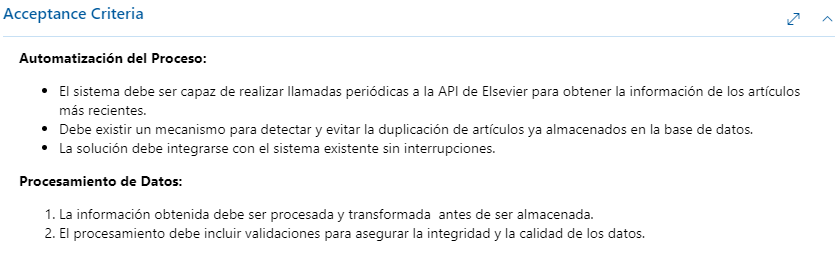
\includegraphics[scale=0.8]{../02Figures/02Chapter/Sprints/Sprint-5/aceptance-criteria-HU-SE-07.png}
    \caption{Criterios de Aceptación HU-SE-07}\label{C2F2:Criterios de Aceptacion HU-SE-07}
\end{figure}

\begin{figure}[H]
    \centering
    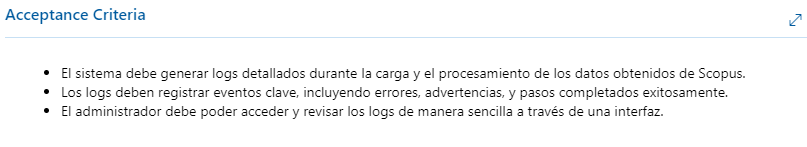
\includegraphics[scale=0.8]{../02Figures/02Chapter/Sprints/Sprint-5/aceptance-criteria-HU-SE-08.png}
    \caption{Criterios de Aceptación HU-SE-08}\label{C2F2:Criterios de Aceptacion HU-SE-08}
\end{figure}

A continuación en la Figura~\ref{fig:azure-board-sprint-5} se muestran las historias de usuario colocadas en Azure DevOps para el Sprint 5.
\begin{figure}[H]
    \centering
    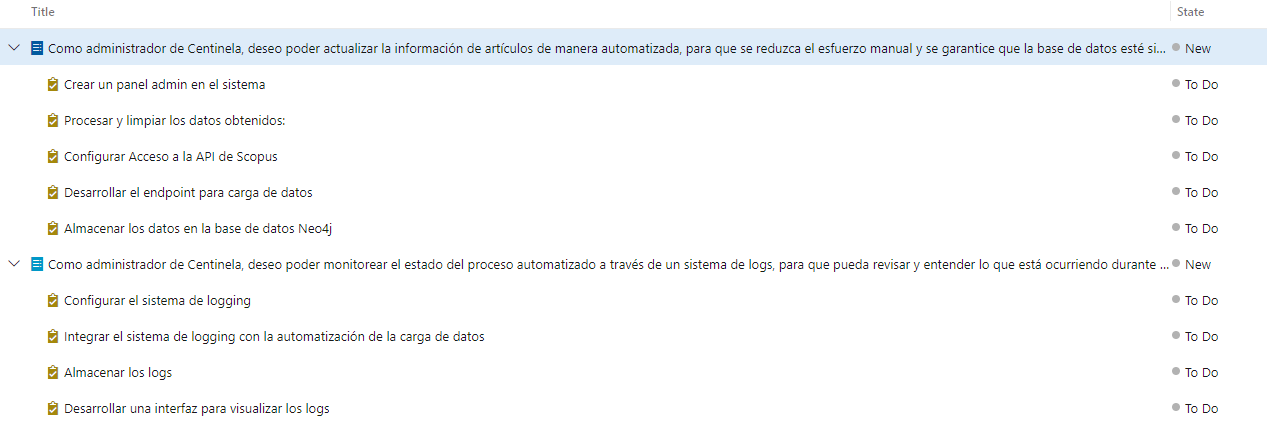
\includegraphics[scale=0.5]{../02Figures/02Chapter/Sprints/Sprint-5/azure-dev-ops-hu-5.png}
    \caption{Historias de Usuario en Azure DevOps para el Sprint 5}\label{fig:azure-board-sprint-5}
\end{figure}

\subsection{Implementación}
Para el desarrollo de este Sprint se ha utilizado la API de Elsevier Scopus~\cite{ElSEVIER} 
para obtener la información de los artículos.
Especificamente dos API's:
\begin{itemize}
    \item \textbf{Search API:} Para obtener la información de los Artículos.
    \item \textbf{Author Retrieval API:} Para obtener la información detallada de los Autores.
\end{itemize}

El flujo de la automatización tanto para extraer la información de los Artículos asi como información detallada sobre un Autor, se puede observar en la Figura~\ref{fig:scopus-automation-flow}.

\begin{figure}[H]
    \centering
    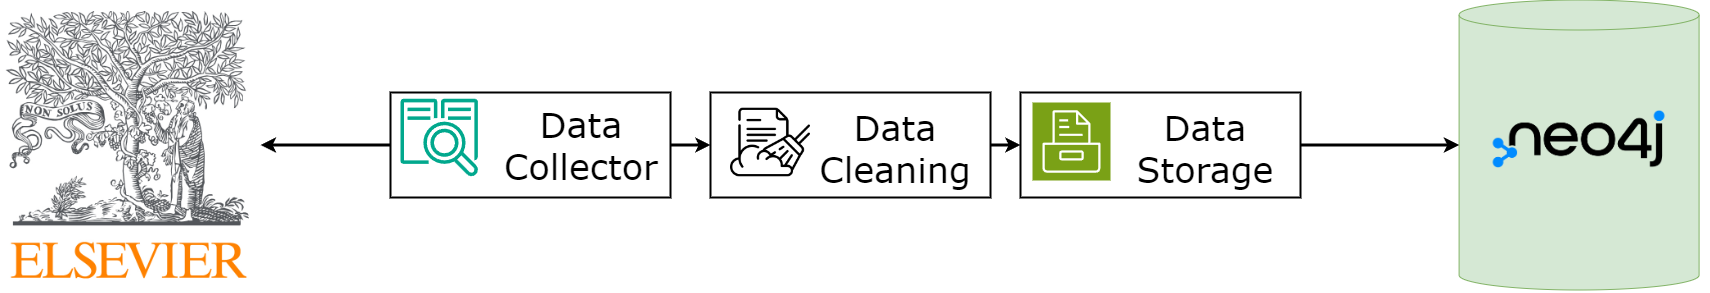
\includegraphics[scale=0.19]{../02Figures/02Chapter/Sprints/Sprint-5/scopus-automation-flow.png}
    \caption{Flujo de la Automatización}\label{fig:scopus-automation-flow}
\end{figure}

El flujo empezará con \textit{Data Collector} que será el encargado de hacer las peticiones a la API de Elsevier,
en esté metodo se analizaran las posib  les respuestas, pero solo si la respuesta tiene un código 200 se procederá a la siguiente fase,
que es el \textit{Data Cleaning} este no es un método, si no un conjunto de reglas definidas. Por ejemplo en la Sección~\ref{chapter02-section02-sprint0}
se mencionó que los modelos van a tener un campo único que permitira identificarlos, el mismo servirá en este caso
para evitar duplicados. Finalmente el proceso de \textit{Data Storage} se encargará de almacenar la información en la base de datos.

Las reglas de limpieza de datos que se han definido son las siguientes:
\begin{itemize}
    \item \textbf{Topic:} El \textit{Topic} debe ser único, por lo que en su campo \textit{name} se ha definido como único.
    \item \textbf{Artículo:} El \textit{Artículo} debe ser único, por lo que sus campos \textit{scopus\_id} y \textit{doi}~\footnote{Digital Object Identifier es un identificador único y permanente para las publicaciones electrónicas} se han definido como únicos.
    \item \textbf{Autor:} El \textit{Autor} debe ser único, por lo que se ha definido su \textit{scopus\_id} como identificador único.
    \item \textbf{Afiliación:} La \textit{Afiliación} debe ser única, por lo que se ha definido su \textit{scopus\_id} como identificador único. Sin embargo, esto no fue suficiente ya que existían muchos datos duplicados con el nombre, por lo que el nombre de la \textit{Afiliación} también pasó a ser único.
\end{itemize}


Para esta Sección, cabe mencionar que se reutilizarón ciertos métodos de Resnet, los mismos que pérmitiran configurar el cliente de la API de Elsevier.

Para la tarea HU-SE-07: Configurar Acceso a la API de Scopus, se ha configurado el cliente de la API de Elsevier, debido a que
este cliente utiliza información sensible, se ha optado por utilizar variables de entorno para almacenar las credenciales de acceso.

En la Figura~\ref{fig:environment-variables} se muestra la estructura del archivo que contendrá las variables de entorno.

\begin{figure}[H]
    \centering
    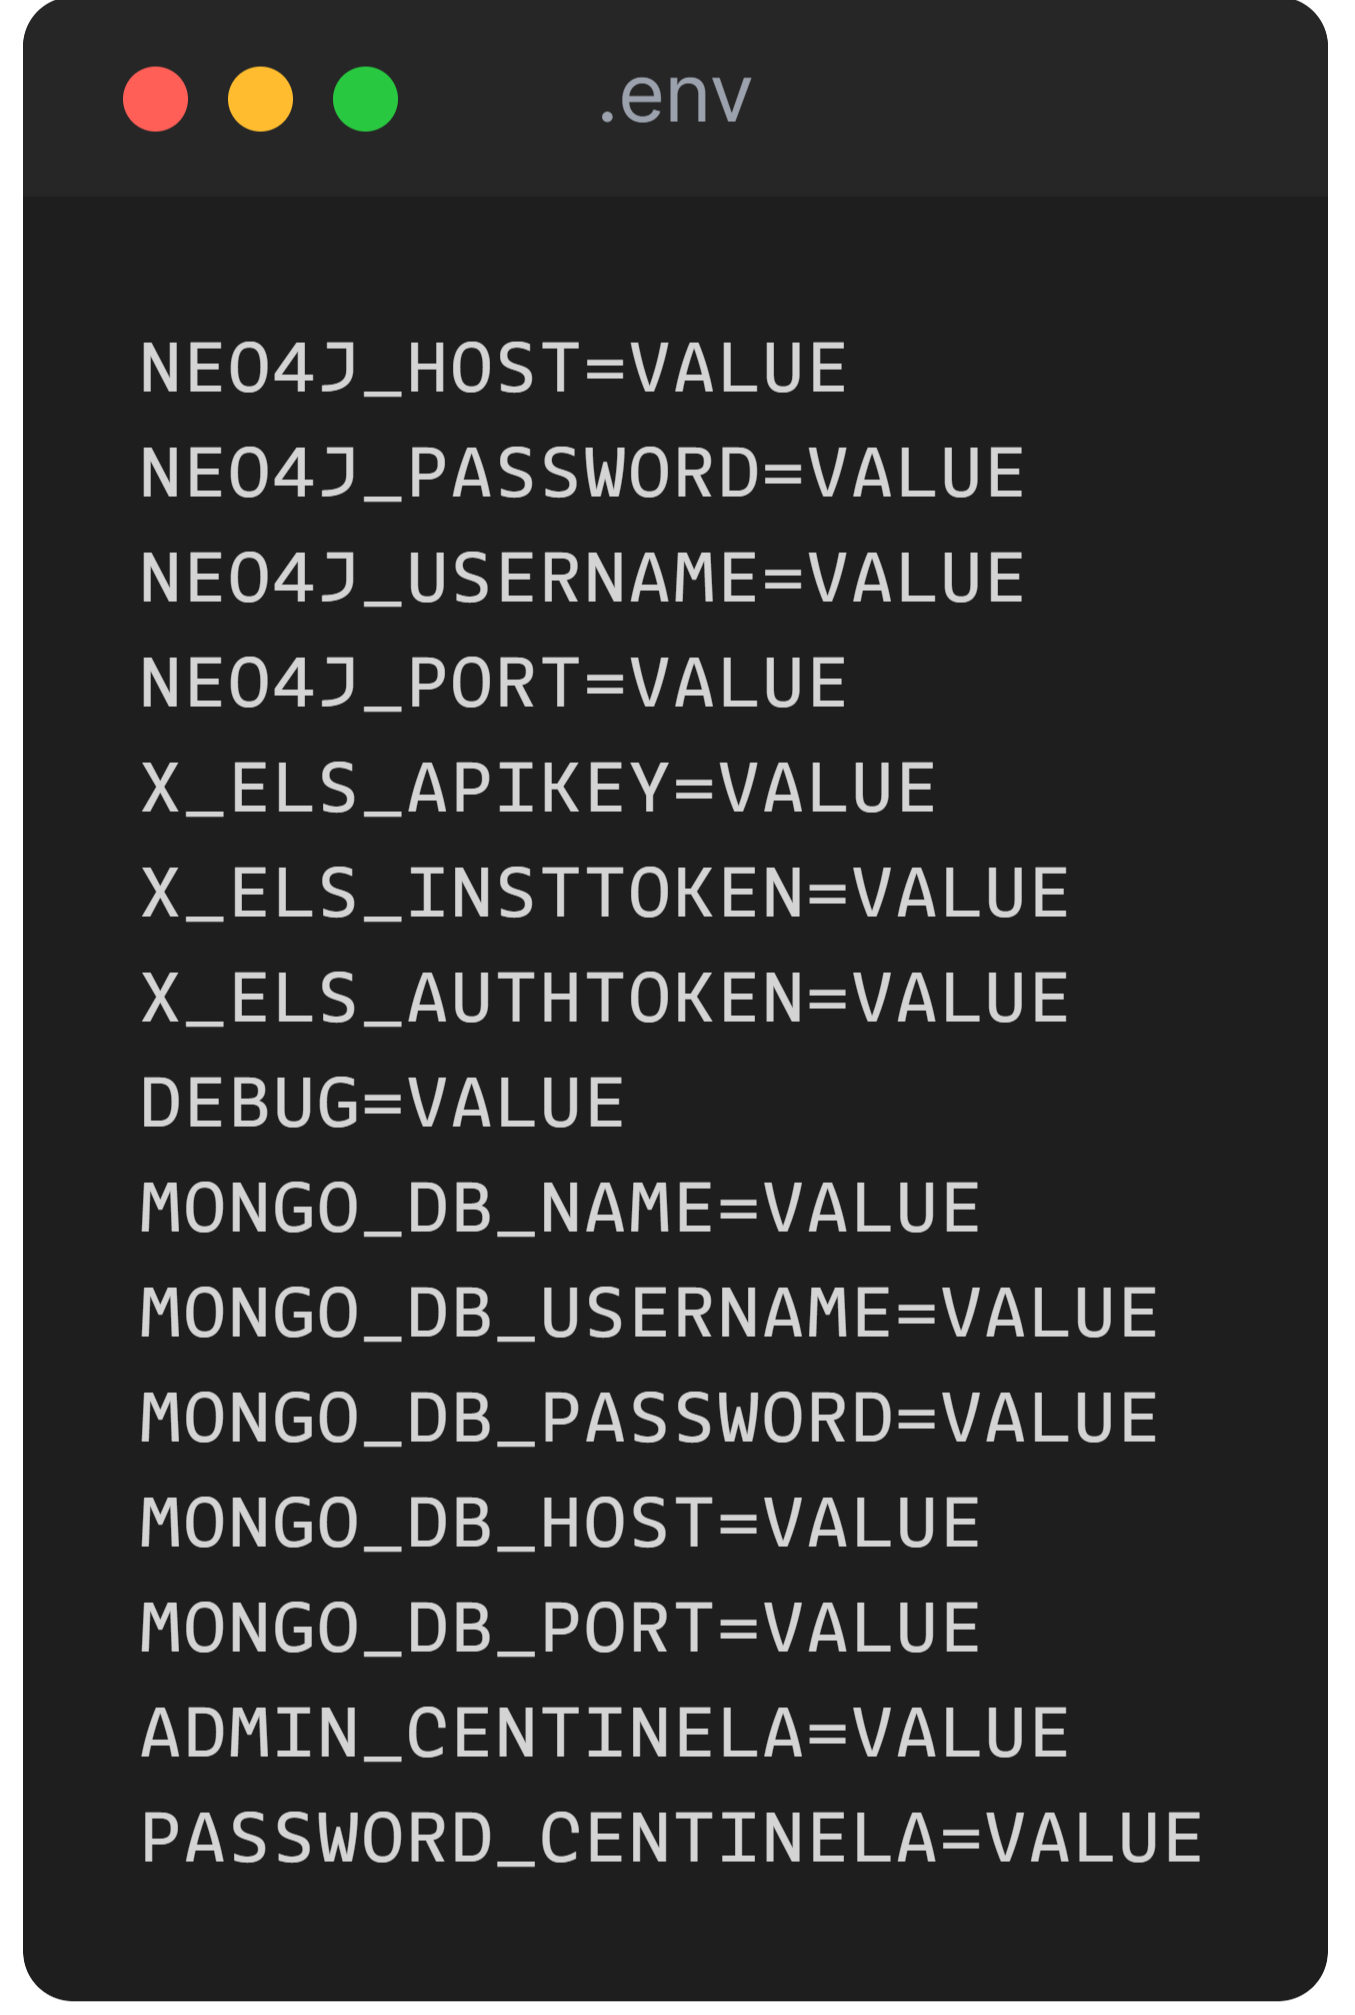
\includegraphics[scale=0.12]{../02Figures/02Chapter/Sprints/Sprint-5/environment-variables.png}
    \caption{Estructura de las Variables de Entorno}\label{fig:environment-variables}
\end{figure}

Para la tarea HU-SE-07: Procesar y limpiar los datos de Scopus, como se menciono anteriormente, se ha definido un conjunto de reglas para limpiar los datos,
al extraer información por ejemplo de un Topic, se ha definido que el mismo debe ser único, por lo que se ha definido un campo único en el modelo,
con la propiedad \textit{\{unique\_index\}} como verdadera. Tambien para este caso especifico se analiza si el topico ya existe caso contrario se crea, a su vez
tiene un método que hace la limpieza del topic previo a guardarlo
como se muestra en la Figura~\ref{fig:topic-model}.

\begin{figure}[H]
    \centering
    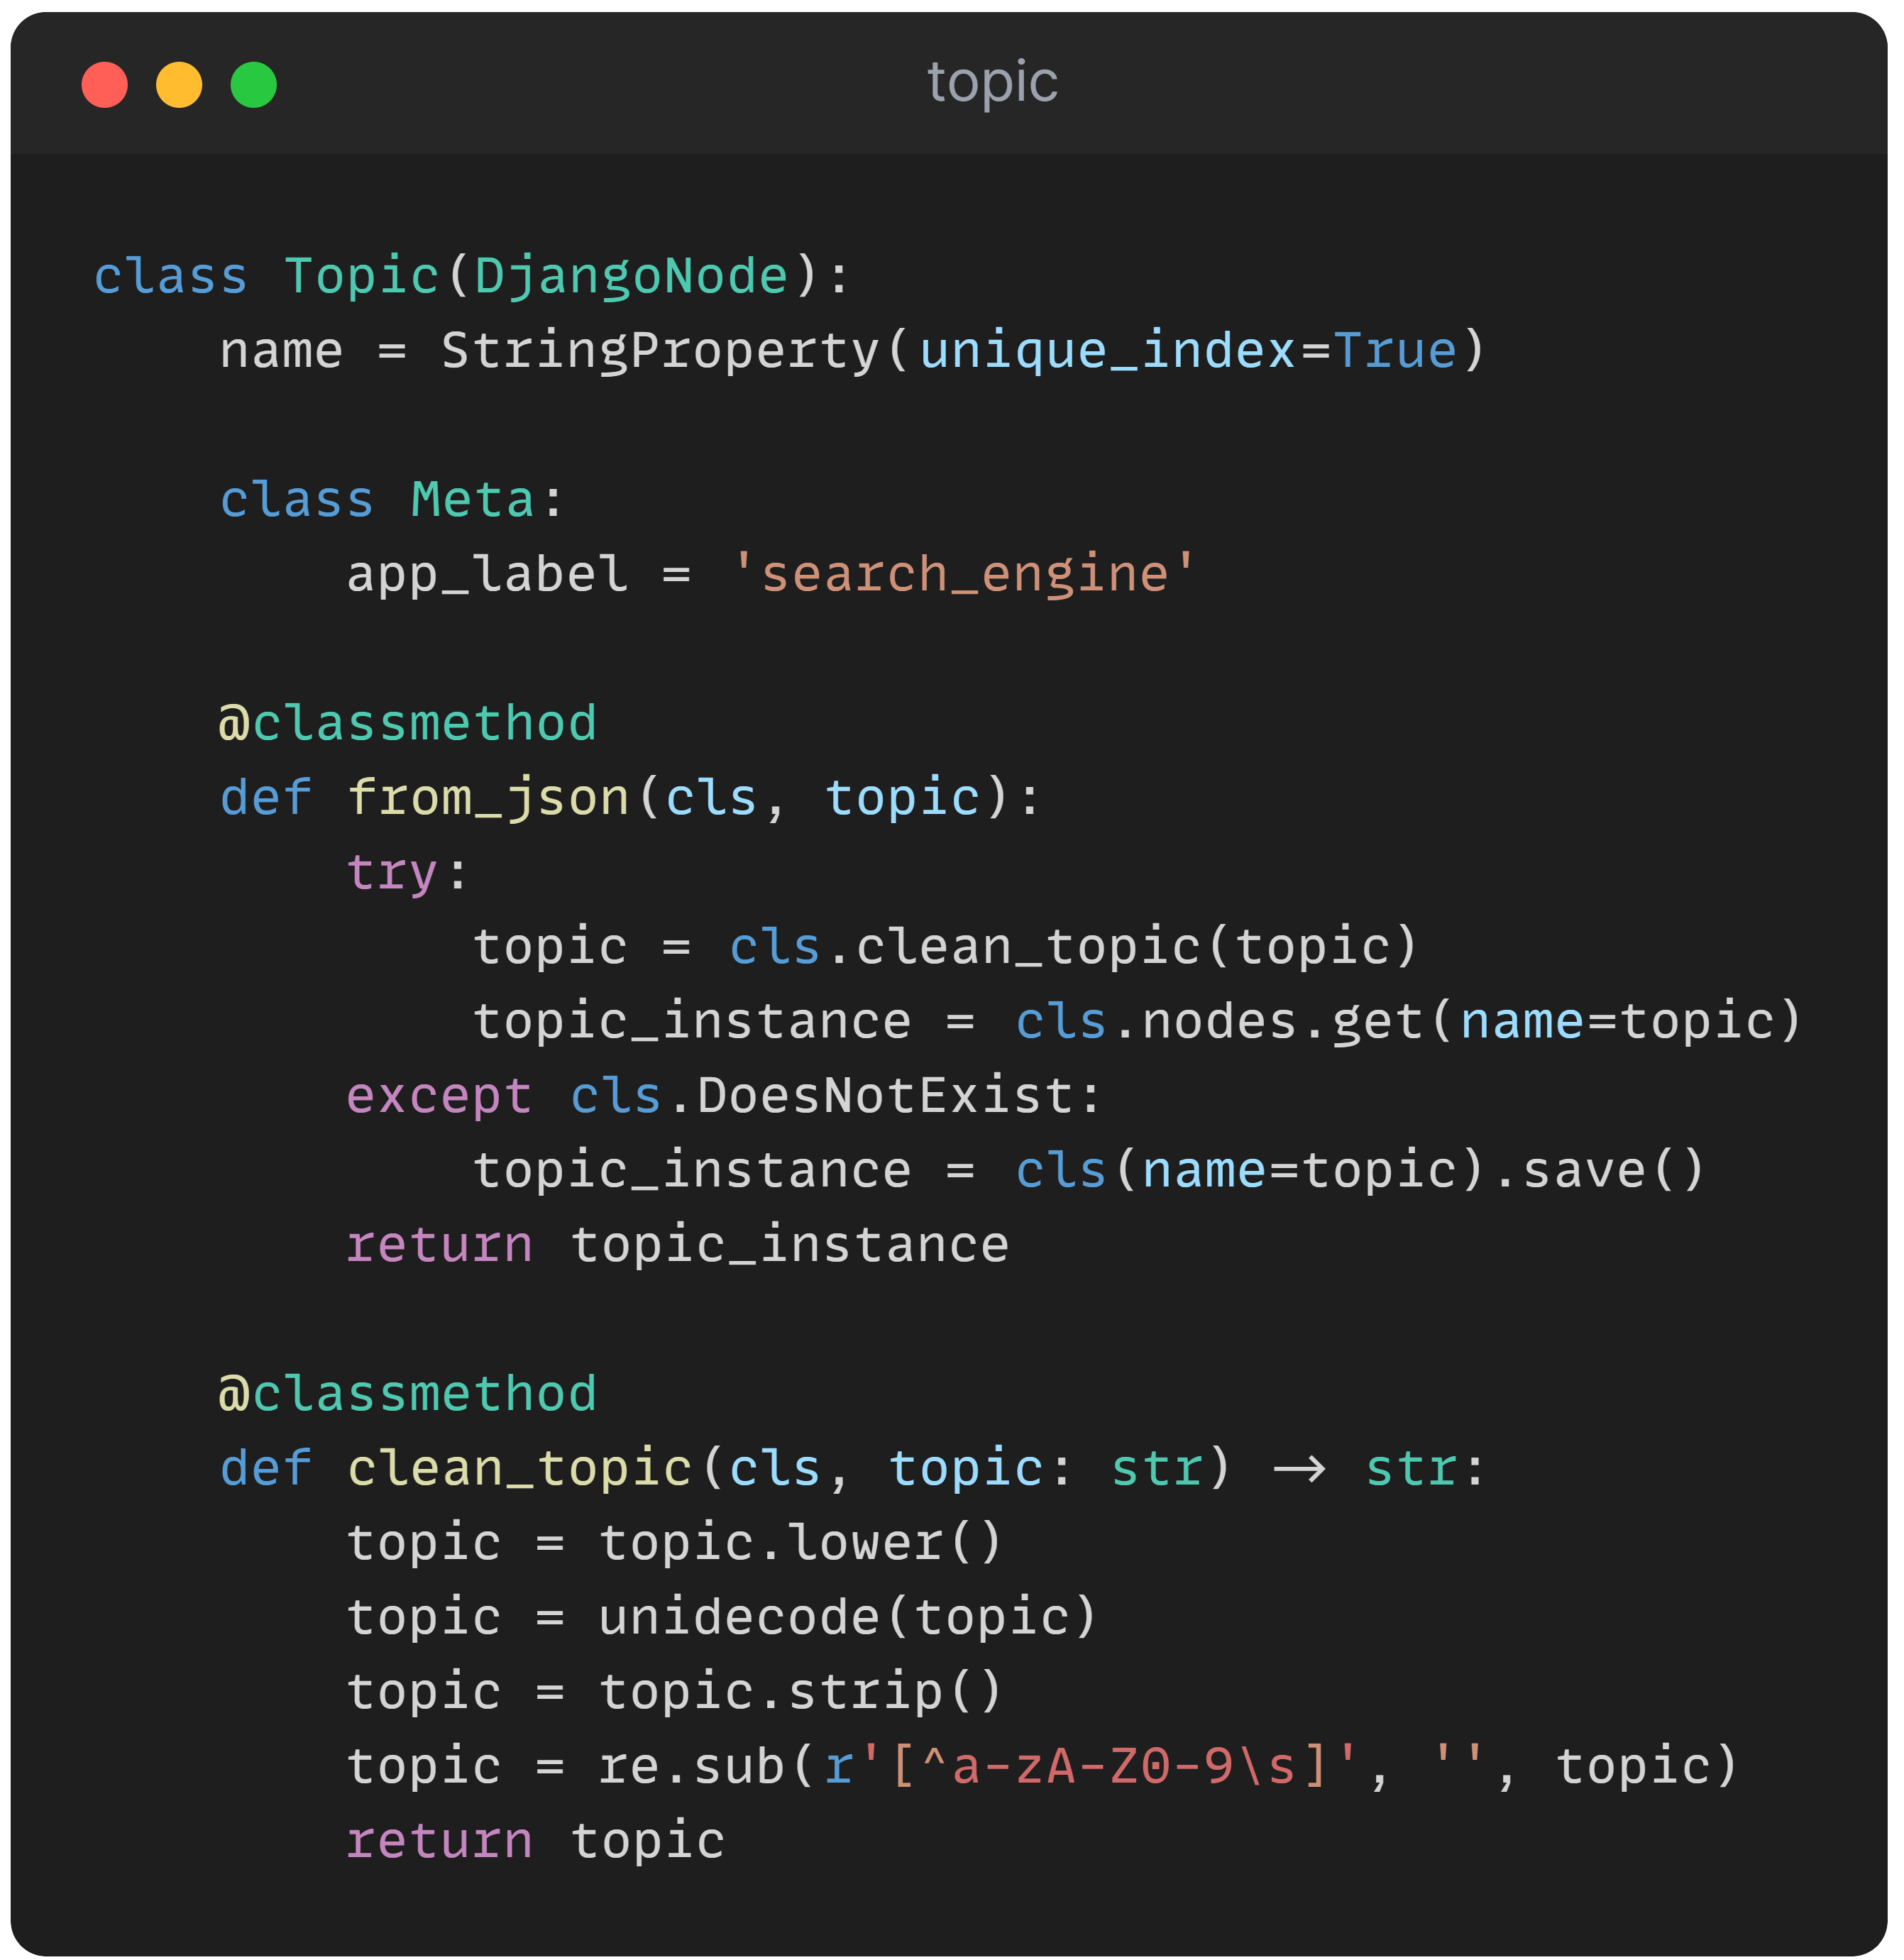
\includegraphics[scale=0.11]{../02Figures/02Chapter/Sprints/Sprint-5/topic-model.png}
    \caption{Modelo Topic}\label{fig:topic-model}
\end{figure}

Para la tarea HU-SE-07: Almacenar los datos en la base de datos Neo4j,
vamos a utilizar como ejemplo la Figura~\ref{fig:topic-model} para mostrar como se almacena la información en la base de datos.
Esta clase tiene un método \texttt{from\_json} que se encarga de guardar la información en la base de datos, en este caso en Neo4j.
Este método es un método de clase, por lo que no es necesario instanciar la clase para poder utilizarlo.
Toda la información que se obtiene de la API de Elsevier es en formato JSON, por lo que se decidió
utilizar este enfoque para facilitar la carga de datos en la base de datos.

Con esto se puede evidenciar como funciona el proceso de extracción, limpieza y carga da datos que provienen desde Scopus.
Este mismo procedmiento es aplicado para todos los modelos de la aplicación.

Para la tarea HU-SE-07: Crear un servicio de búsqueda de Artículos, se reutilizó la misma lógica de Resnet.
Con la diferencia que en este caso al llegar la información en formato JSON, nos permite acceder a esos datos
y guardarlos en la base de datos, haciendo referencia al flujo mencionado anteriormente.

En la Figura~\ref{fig:sequence-diagram-scopus-integration} se muestra un diagrama de secuencia de como se integra la API de Elsevier con la aplicación.
La interacción empieza cuando el usuario hace una peticion al endpoint \texttt{/api/v1/scopus-integration/} (GET) para buscar los Artículos que tengan algúna Afiliación en Ecuador.
La vista \texttt(ScopusIntegrationView) llama al caso de uso \texttt{ScopusIntegrationUseCase} que a su vez llama al repositorio \texttt{SearchAffiliationUseCase}.
Este repositorio se encarga de hacer la petición a la API de Elsevier y devolver la información en formato JSON\@.
La misma que es procesada y almacenada en la base de datos. Finalmente se tiene un \texttt(ModelCorpusObserver), el que se encargará de eliminar los archivos Pickle tanto el Corpus como el Modelo ya que con nueva información
ambos deben ser generados nuevamente.

\begin{figure}[H]
    \centering
    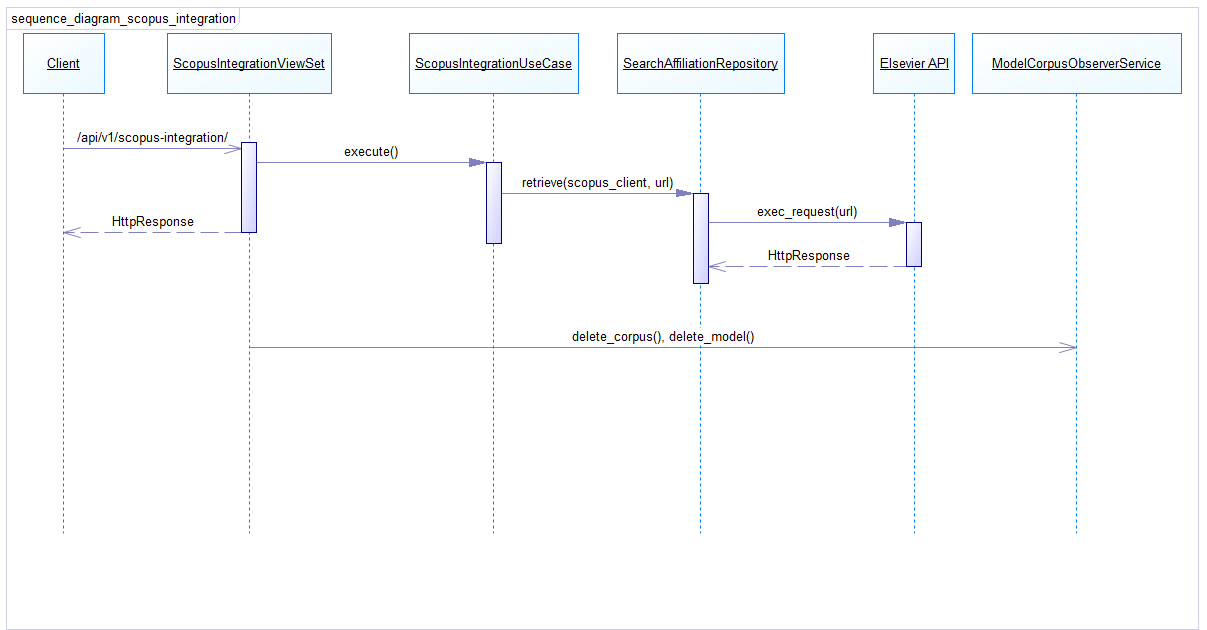
\includegraphics[scale=0.5]{../02Figures/02Chapter/Sprints/Sprint-5/sequence_diagram_scopus_integration.png}
    \caption{Diagrama de Secuencia de la Integración con la API de Elsevier}\label{fig:sequence-diagram-scopus-integration}
\end{figure}

Entre otra información, para cada Artículo que devuelve la busqueda en Elsevier, se obtiene la información general del Articulo,
Afiliaciones, Autores, entre otros como se puede ver en la Figura~\ref{fig:article-json}.
\begin{figure}[!ht]
    \centering
    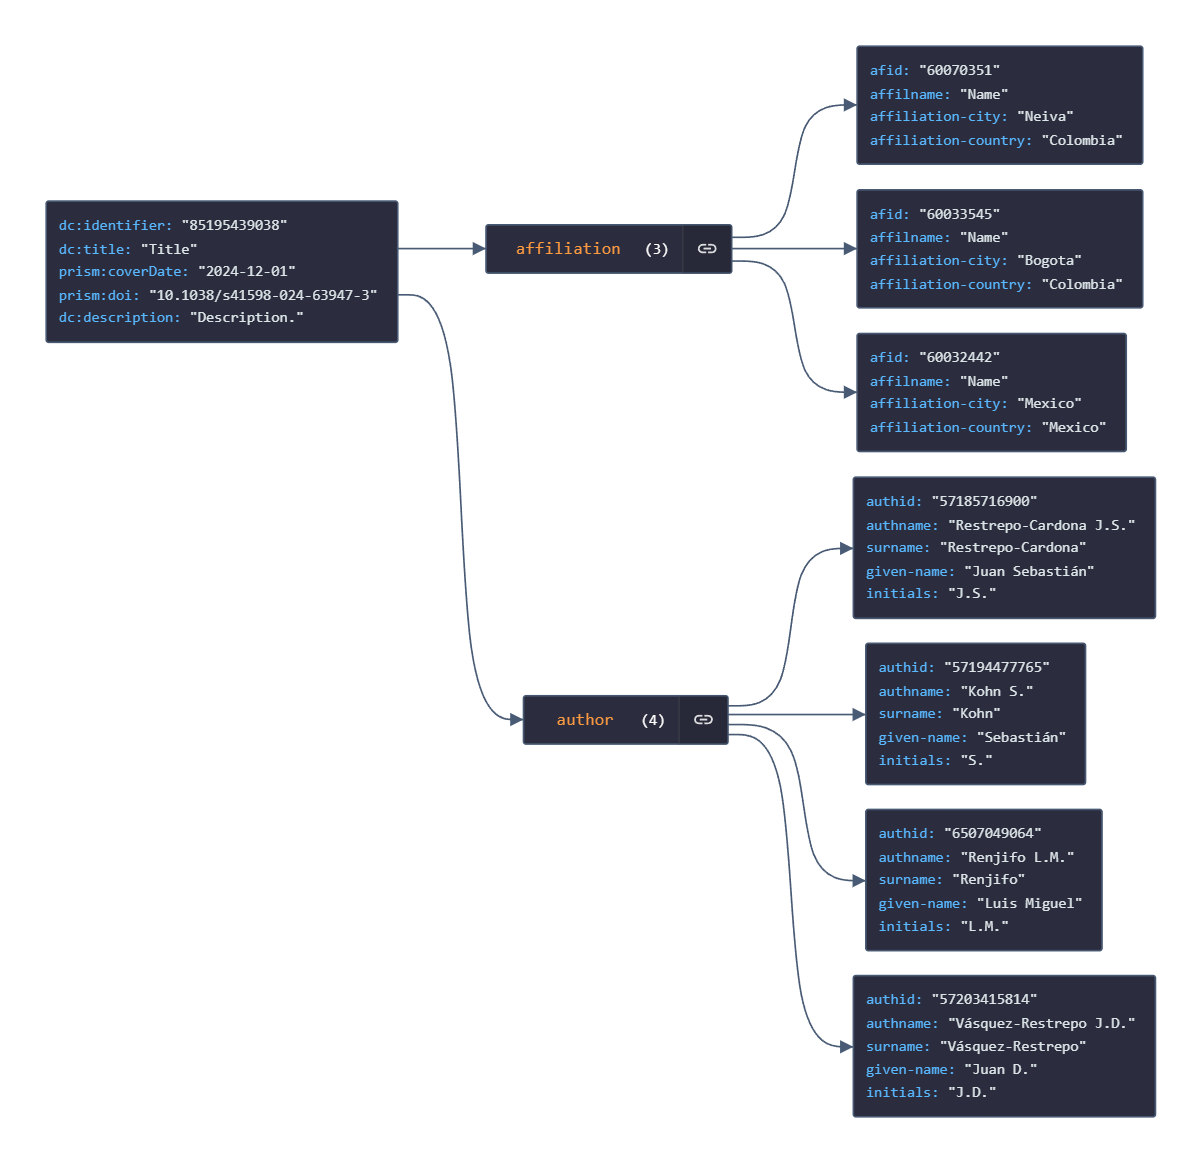
\includegraphics[scale=0.3]{../02Figures/02Chapter/Sprints/Sprint-5/article_json.png}
    \caption{Ejemplo de JSON de un Artículo}\label{fig:article-json}
\end{figure}

Debido a esto, se identificó un problema. Si bien la información referente a los autores nos permite armar las redes de coautoría, esta información no es suficienta para los intereses de Centinela.
Por lo que se decidió utilizar la API de  Author Retrieval para obtener la información detallada de los autores.

Para la tarea HU-SE-07: Implementar el servicio para obtener la información detallada de los Autores, se ha utilizado la API de Author Retrieval de Elsevier.
De igual manera la información que se obtiene es en formato JSON~\footnote{Javascript Object Notation, archivo con datos estructurados que se utiliza para comunicar aplicaciones}, el enfoque presentado anteriormente es aplicado en este caso.
Dado que la información que se obtiene de la API de Author Retrieval es muy extensa, no se ha podido mostrar un ejemplo de la misma.
Sin embargo se puede consultar en la documentación de Elsevier~\cite{ElSEVIER}.

El diagrama de secuencia de la integración con la API de Author Retrieval se muestra en la Figura~\ref{fig:sequence-diagram-author-retrieval}.


El mismo que muestra información general sobre el estado de Centinela. Por ejemplo cuantos Artículos y Autores se han almacenado en la base de datos.
Y una comparación de los mismmos con la información que se obtiene de la API de Elsevier.
De igual manera se tiene una sección para actualizar el corpus y el modelo.


De manera similar al diagrama de secuencia de la integración con la API de Elsevier, el flujo empieza con el usuario haciendo una petición al endpoint \url{/api/v1/author-retrieval/} (GET)
para buscar la información detallada de un Autor.
La vista \texttt{AuthorRetrievalView} llama al caso de uso \texttt{AuthorRetrievalUseCase} que a su vez llama al repositorio \texttt{AuthorRetrievalRepository}.
Este repositorio se encarga de hacer la petición a la API de Author Retrieval y devolver la información en formato JSON\@.
La misma que es procesada y almacenada en la base de datos. Nuevamente el Corpus y el Modelo son eliminados para ser generados nuevamente.

\begin{figure}[H]
    \centering
    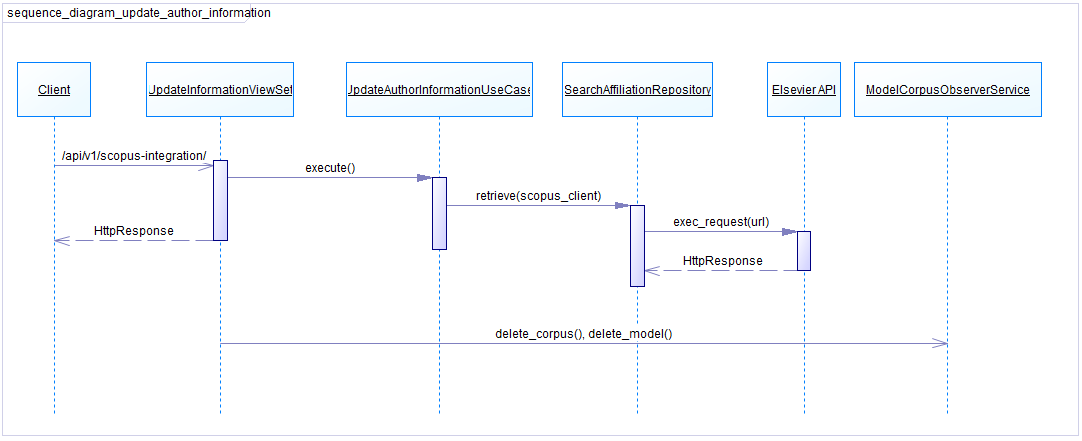
\includegraphics[scale=0.6]{../02Figures/02Chapter/Sprints/Sprint-5/sequence_diagram_update_author_information.png}
    \caption{Diagrama de Secuencia de la Integración con la API de Author Retrieval}\label{fig:sequence-diagram-author-retrieval}
\end{figure}



Una vez que se ha desarrollado estas funcionalidades, el siguiente paso es dar un punto de entrada.
Para esto se ha desarrollado un panel de administración, que permitirá al administrador actualizar la información de los Artículos y Autores de manera automatizada.


Para la tarea HU-SE-08: Configurar un sistema de logging, se ha utilizado la librería \texttt{logging} de Python, la misma que permite almacenar los logs en un archivo.
En la Figura~\ref{fig:logging} se muestra un ejemplo de como se configura el sistema de logging.

\begin{figure}[H]
    \centering
    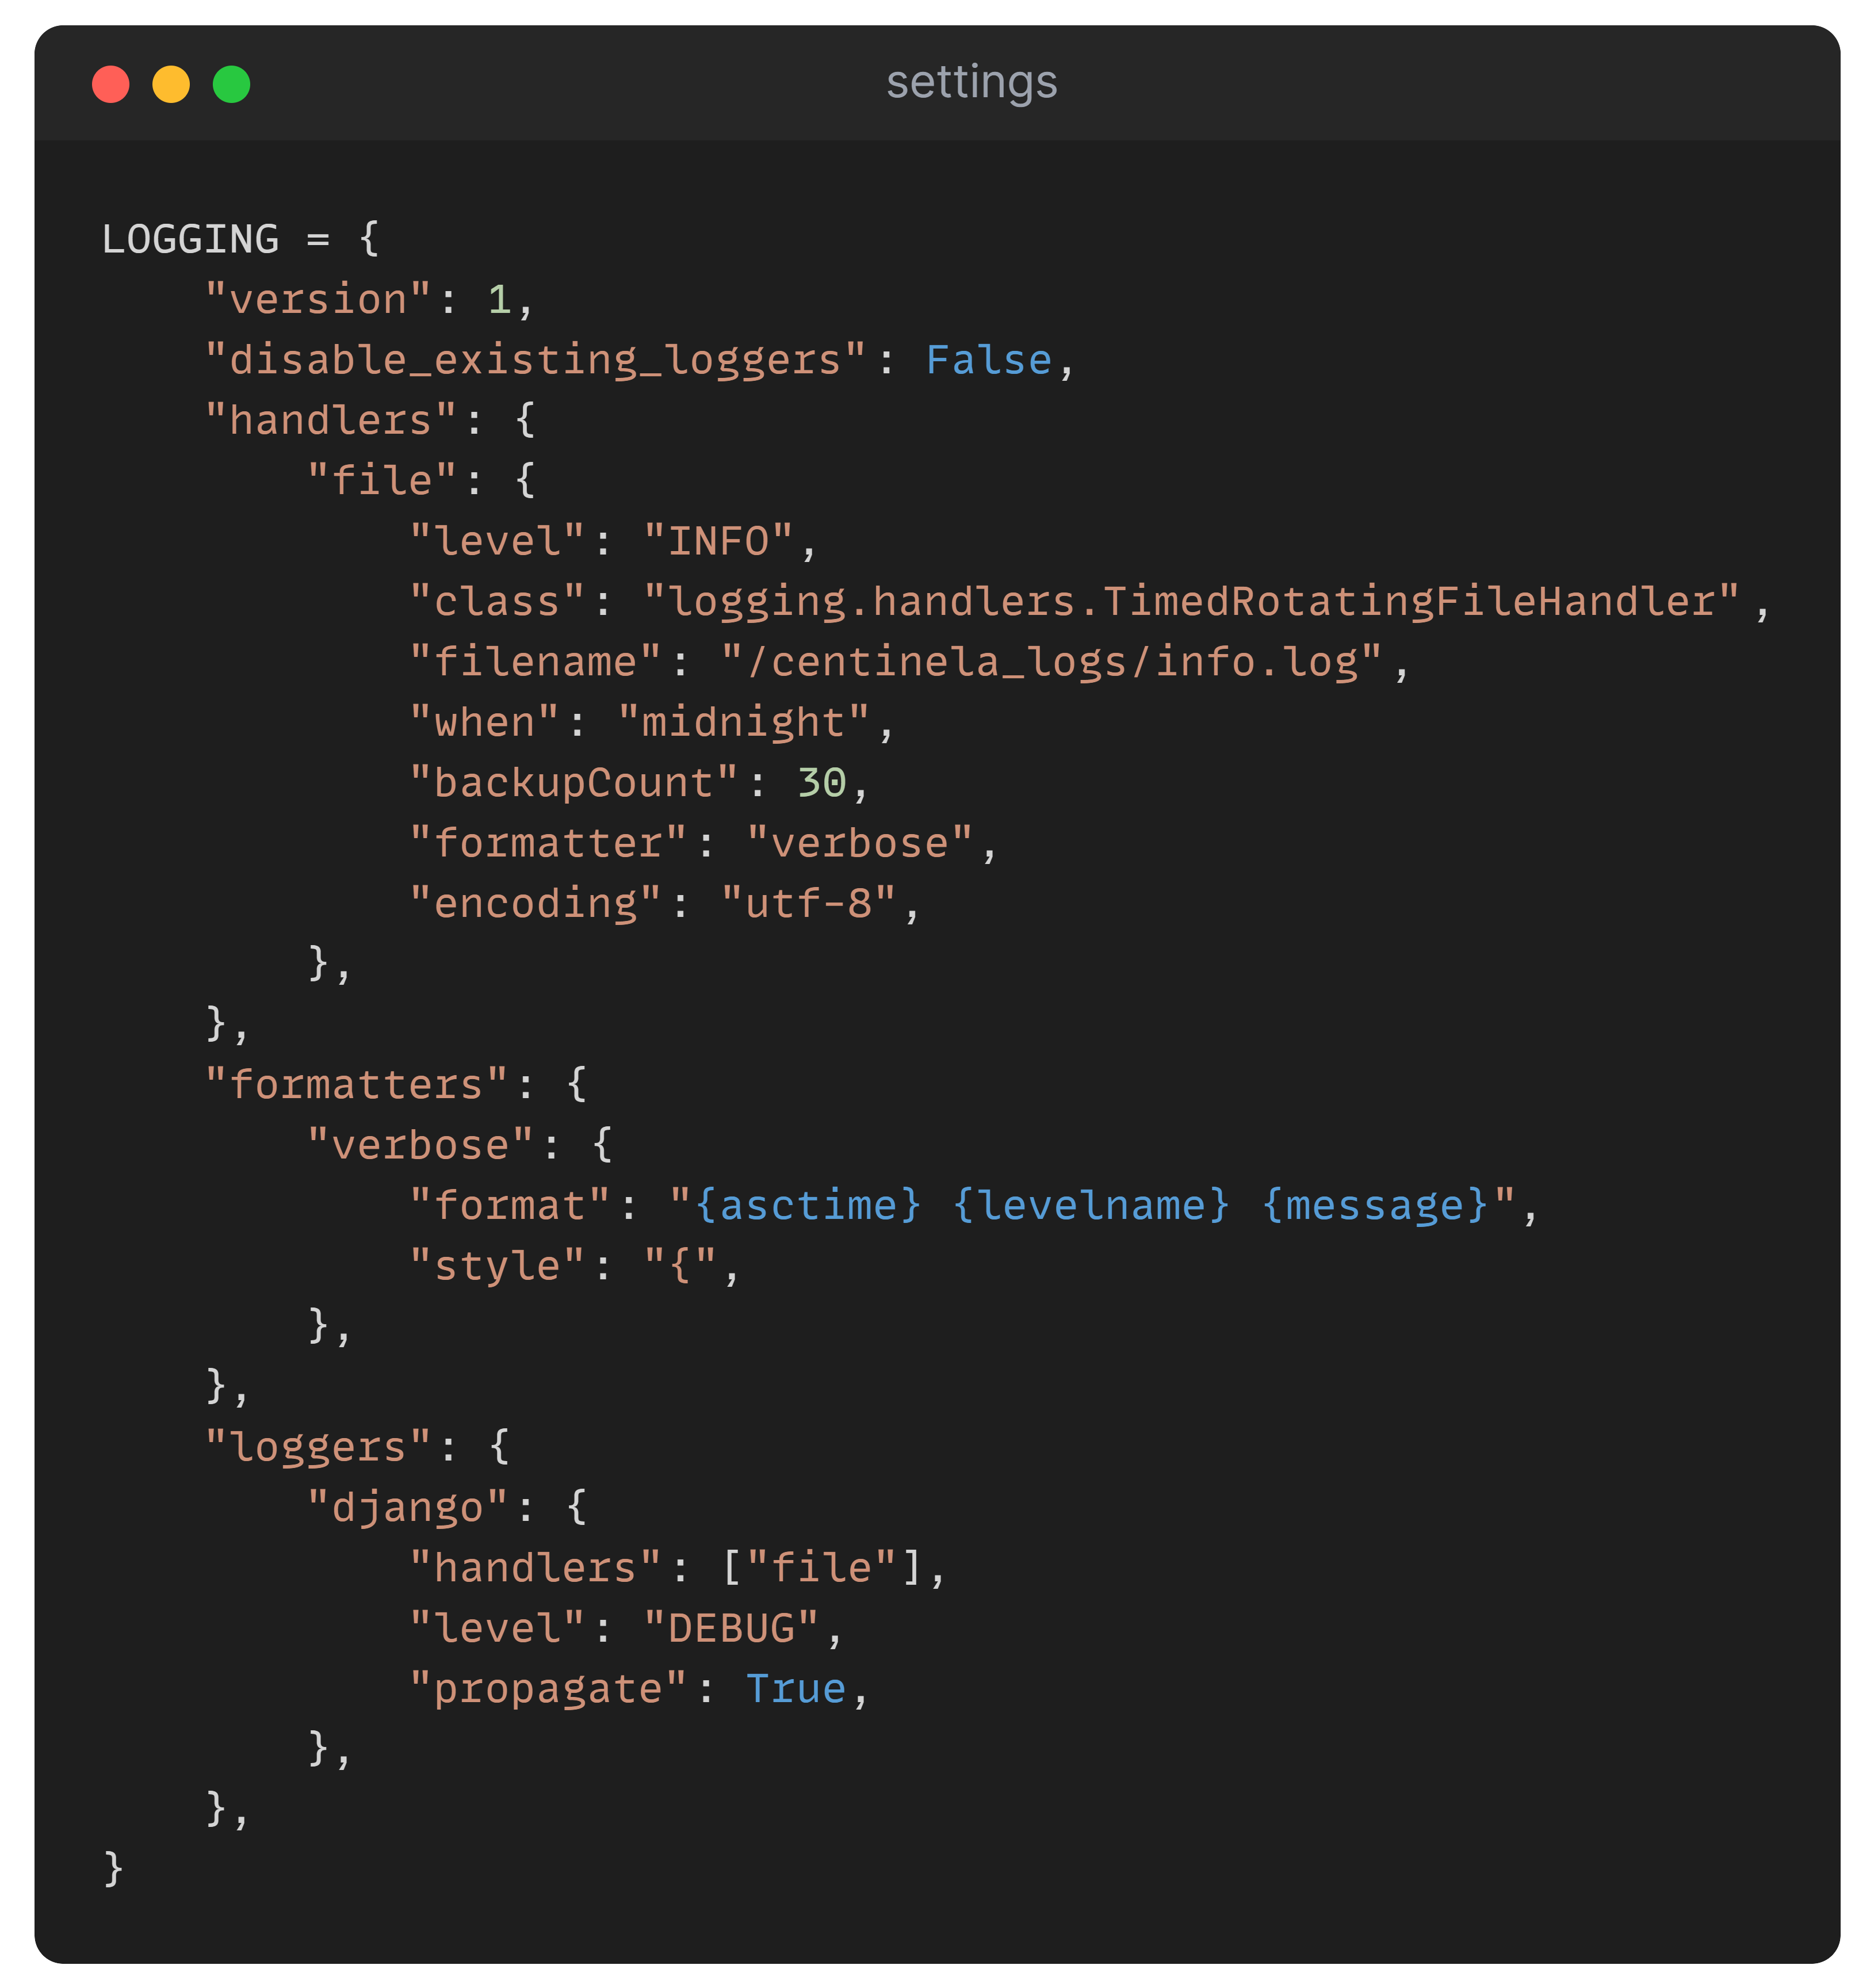
\includegraphics[scale=0.15]{../02Figures/02Chapter/Sprints/Sprint-5/logging.png}
    \caption{Configuración del Sistema de Logging}\label{fig:logging}
\end{figure}

La configuración mostrada en la Figura~\ref{fig:logging} permite almacenar los logs en un archivo, con rotación diaria a medianoche y conservación de hasta 30 archivos de respaldo.
Los mensajes se formatean incluyendo la fecha y hora, el nivel del registro y el mensaje en sí.
El nivel del registro que se consideró fue \texttt{INFO}, debido a que es el nivel que ofrece información relevante sobre el proceso, pero se puede cambiar a \texttt{DEBUG} para obtener más información.

Finalmente para la tarea HU-SE-07: Crear un panel admin para actualizar la información de los Artículos y Autores, se ha creado un Login previo para 
que únicamente el administrador de Centinela pueda acceder a dicho panel. El login se muestra en la Figura~\ref{fig:login-admin}.
\begin{figure}[H]
    \centering
    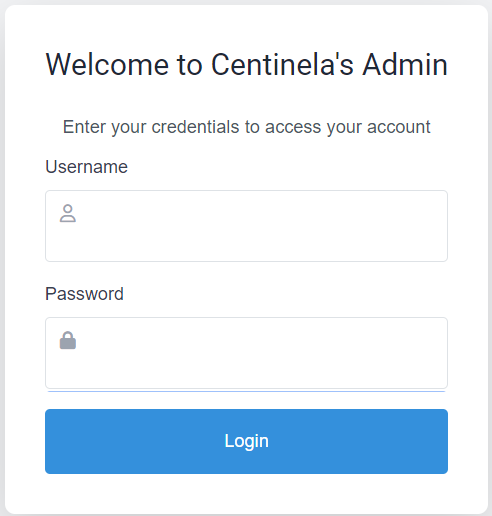
\includegraphics[scale=0.6]{../02Figures/02Chapter/Sprints/Sprint-5/centinela-admin.png}
    \caption{Login de Administrador}\label{fig:login-admin}
\end{figure}

Dado que ese un sistema de Autenticación y Autorización esta fuera de el alcance de este componente
se ha optado por utilizar un sistema de autenticación básico, que consiste en un usuario y contraseña que se almacenan en variables de entorno que se muestran en la Figura~\ref{fig:environment-variables}.

Una vez autenticado el administrador, se le presentará el panel que se muestra en la Figura~\ref{fig:admin-panel}.
\begin{figure}[H]
    \centering
    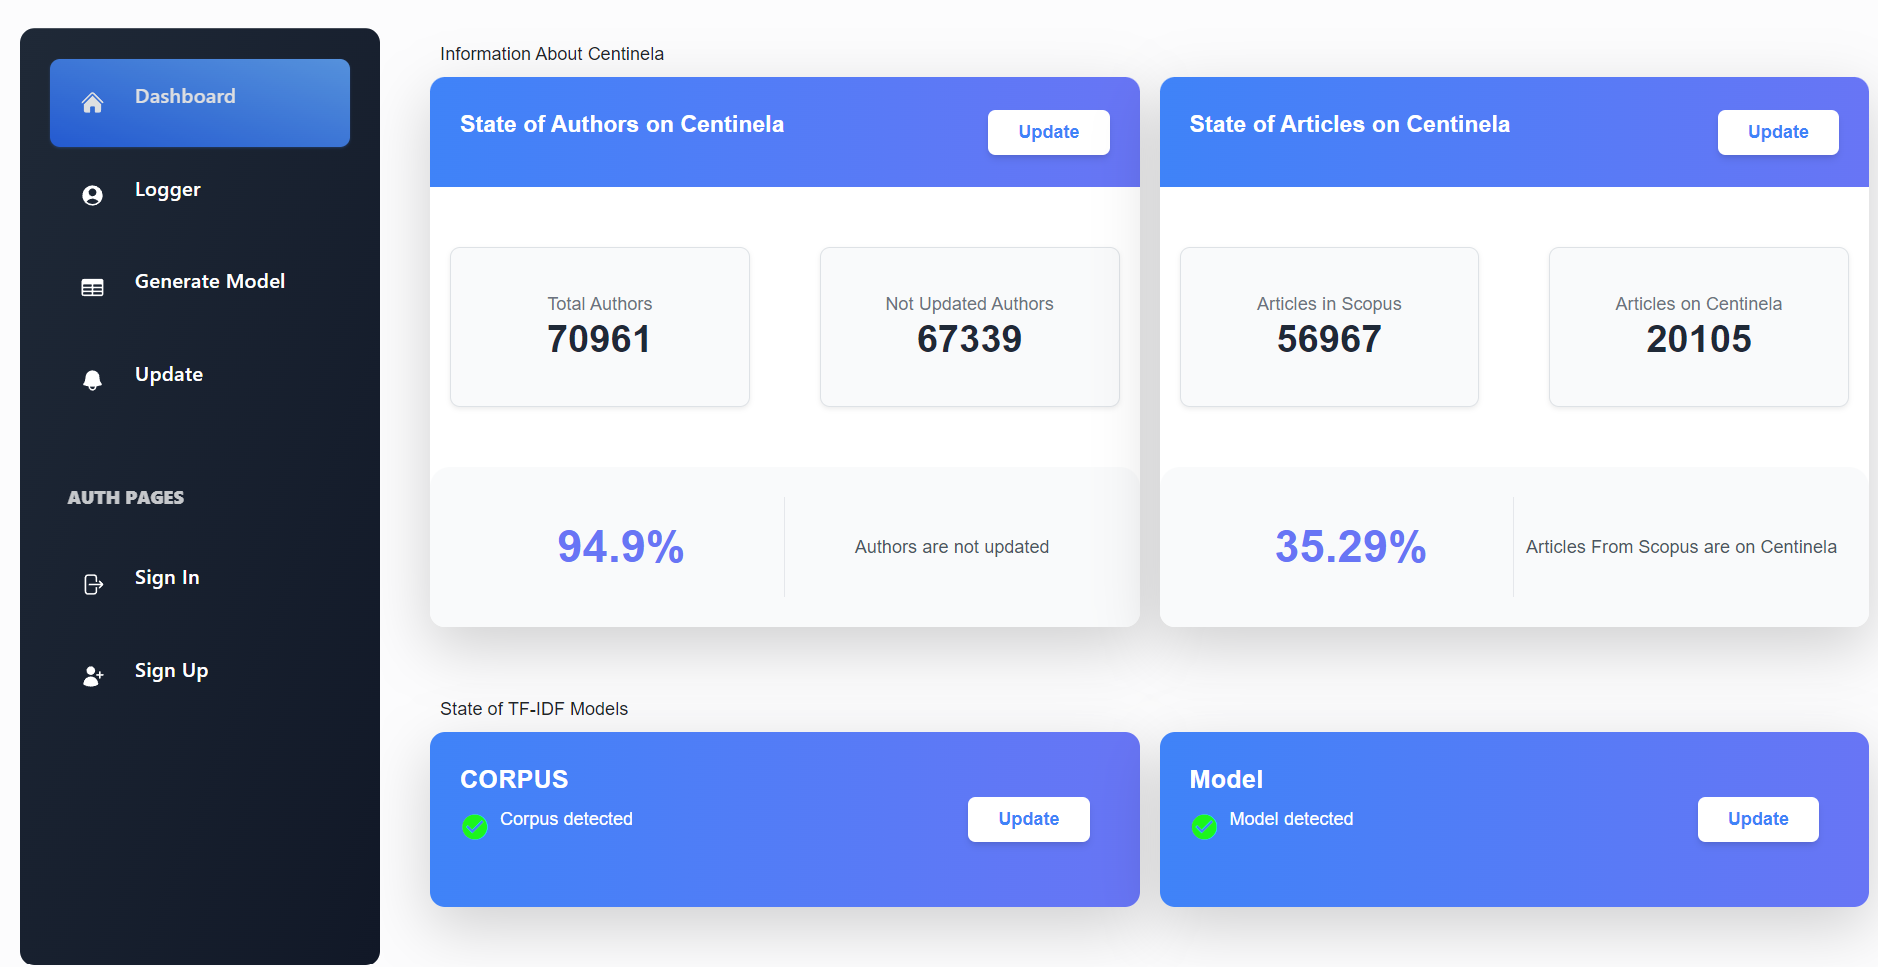
\includegraphics[scale=0.34]{../02Figures/02Chapter/Sprints/Sprint-5/admin-panel.png}
    \caption{Panel de Administración}\label{fig:admin-panel}
\end{figure}

El mismo que muestra información general sobre el estado de Centinela. Por ejemplo cuantos Artículos y Autores se han almacenado en la base de datos.
Y una comparación de los mismmos con la información que se obtiene de la API de Elsevier.
De igual manera se tiene una sección para actualizar el corpus y el modelo.

La otra sección es el panel en donde se pueden observar los logs de la aplicación, como se muestra en la Figura~\ref{fig:logs-panel}.
El mismo cuenta con una interfaz que permite filtrar los logs por nivel, fecha o palabra clave.
\begin{figure}[H]
    \centering
    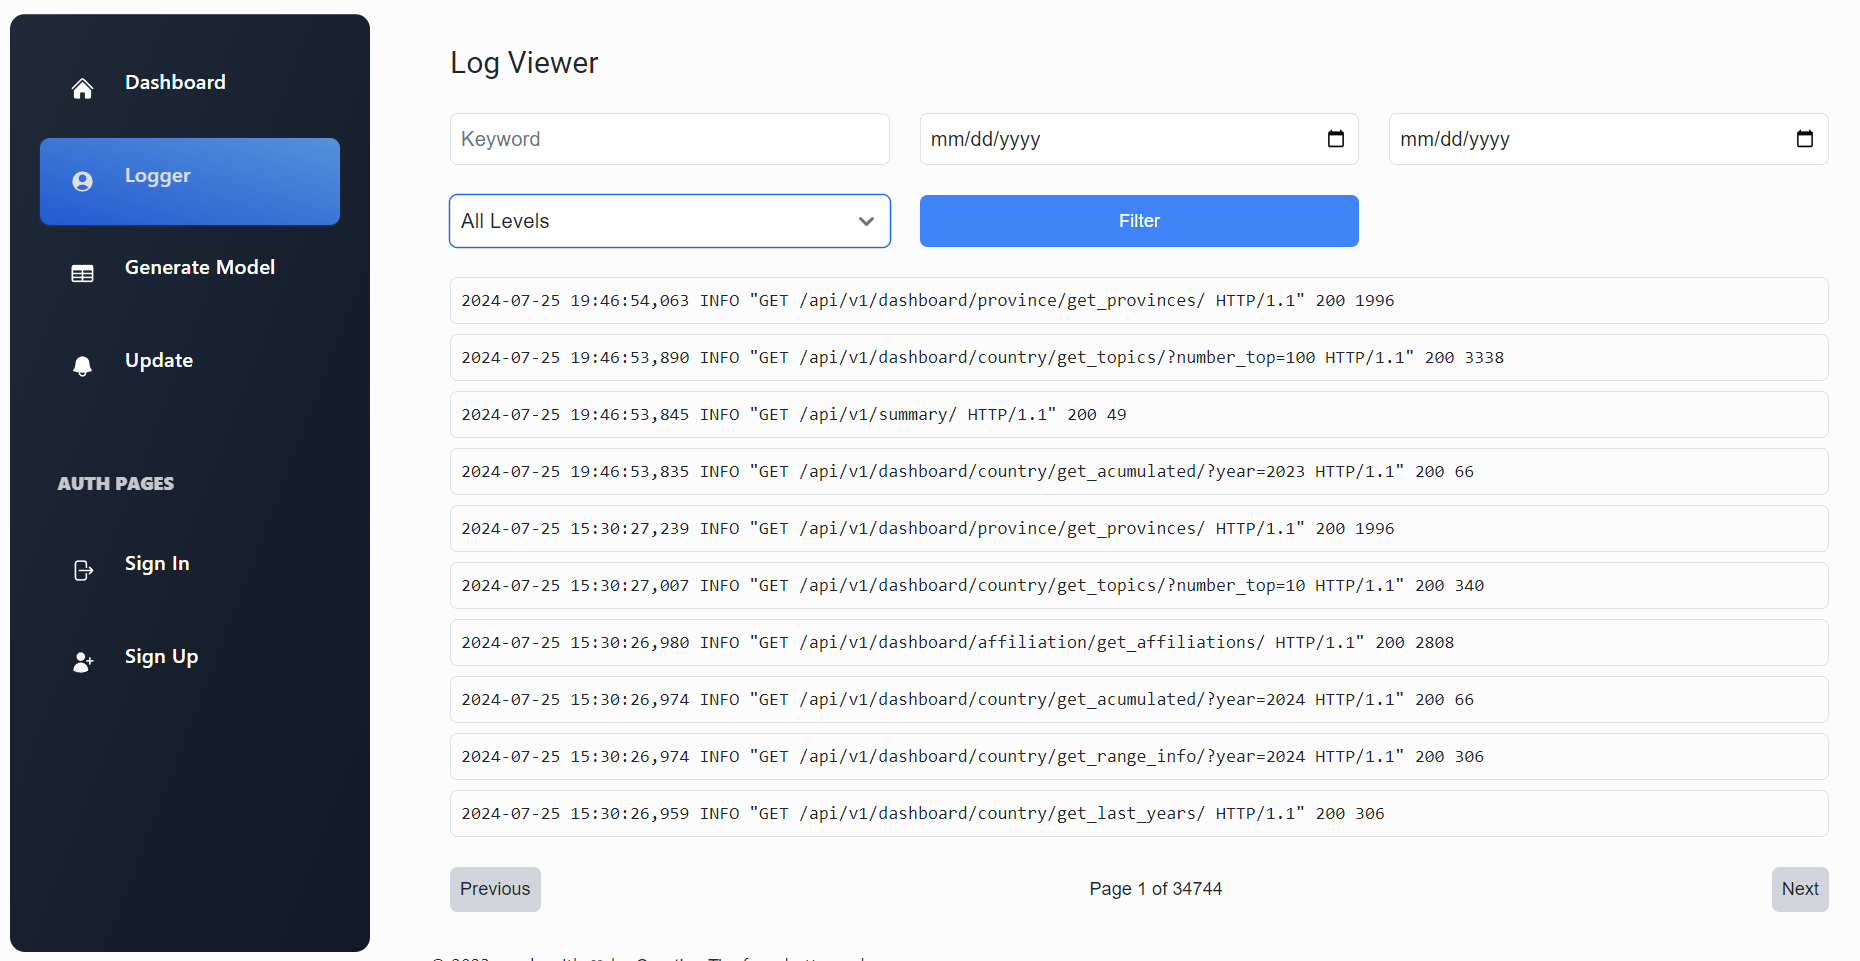
\includegraphics[scale=0.37]{../02Figures/02Chapter/Sprints/Sprint-5/logs-panel.png}
    \caption{Panel de Logs}\label{fig:logs-panel}
\end{figure}



\subsection{Revisión y Retrospectiva}
Al finalizar el Sprint 5, se ha logrado implementar la automatización para la extracción de datos de Scopus, la automatización para la carga de datos de Scopus en Neo4j y el sistema de monitoreo para la automatización de la extracción, limpieza y carga de datos de Scopus.
Se ha logrado cumplir con los objetivos planteados en la planificación del Sprint.
Sin embargo la base de datos aun no cuenta con toda la información que genera las consultas a la API de Elsevier, esto debido a que la información que se obtiene de la API de Elsevier es muy extensa y se requiere de un mayor tiempo para poder procesarla y almacenarla en la base de datos.
Ademas que las credenciales de acceso a la API tienen reestricciones semenales que limitan la cantidad de información que se puede obtener.
